\documentclass[tikz,14pt,border=10pt]{standalone}

\usepackage{verbatim}

\usepackage{textcomp}
\usepackage{amsmath}
\renewcommand{\vec}[1]{\boldsymbol{#1}}
\usetikzlibrary{shapes,arrows,positioning}
\usetikzlibrary{calc,patterns,decorations.pathmorphing,decorations.markings}
\begin{document}
% Definition of blocks:
\tikzset{%
  block_s/.style    = {draw, thick, rectangle, minimum height = 3em,
    minimum width = 3em},
  block_b/.style    = {draw, thick, rectangle, minimum height = 5em,
    minimum width = 8em},
  block_d/.style    = {draw, dash dot, rectangle, minimum height = 5em,
    minimum width = 8em},
  sum/.style      = {draw, circle, node distance = 2cm}, % Adder
  input/.style    = {coordinate}, % Input
  output/.style   = {coordinate}, % Output
  anch/.style   = {coordinate} % Anchor
}
% Defining string as labels of certain blocks.
\newcommand{\suma}{}

\begin{tikzpicture}[auto, thick, node distance=2cm, >=triangle 45]
  \draw
  node[input, name = diagram_init]{}
  
  node[block_d, right = 40 pt of diagram_init, align=center] (high_level_p){High-Level \\ Planner}
  node[anch, below = 15pt of high_level_p.east] (p_des_anchor_left){}
  
  node[block_b, right = 40 pt of high_level_p, align=center] (hic){Hybrid Impedance \\Controller}
  node[anch, below = 15pt of hic.west] (p_des_anchor_right){}
  
  node[block_b, right = 40 pt of hic, align=center] (op_space_inv_d){Operational Space \\ Inverse Dynamics \\ Controller}
  node[block_b, right = 40 pt of op_space_inv_d] (kuka){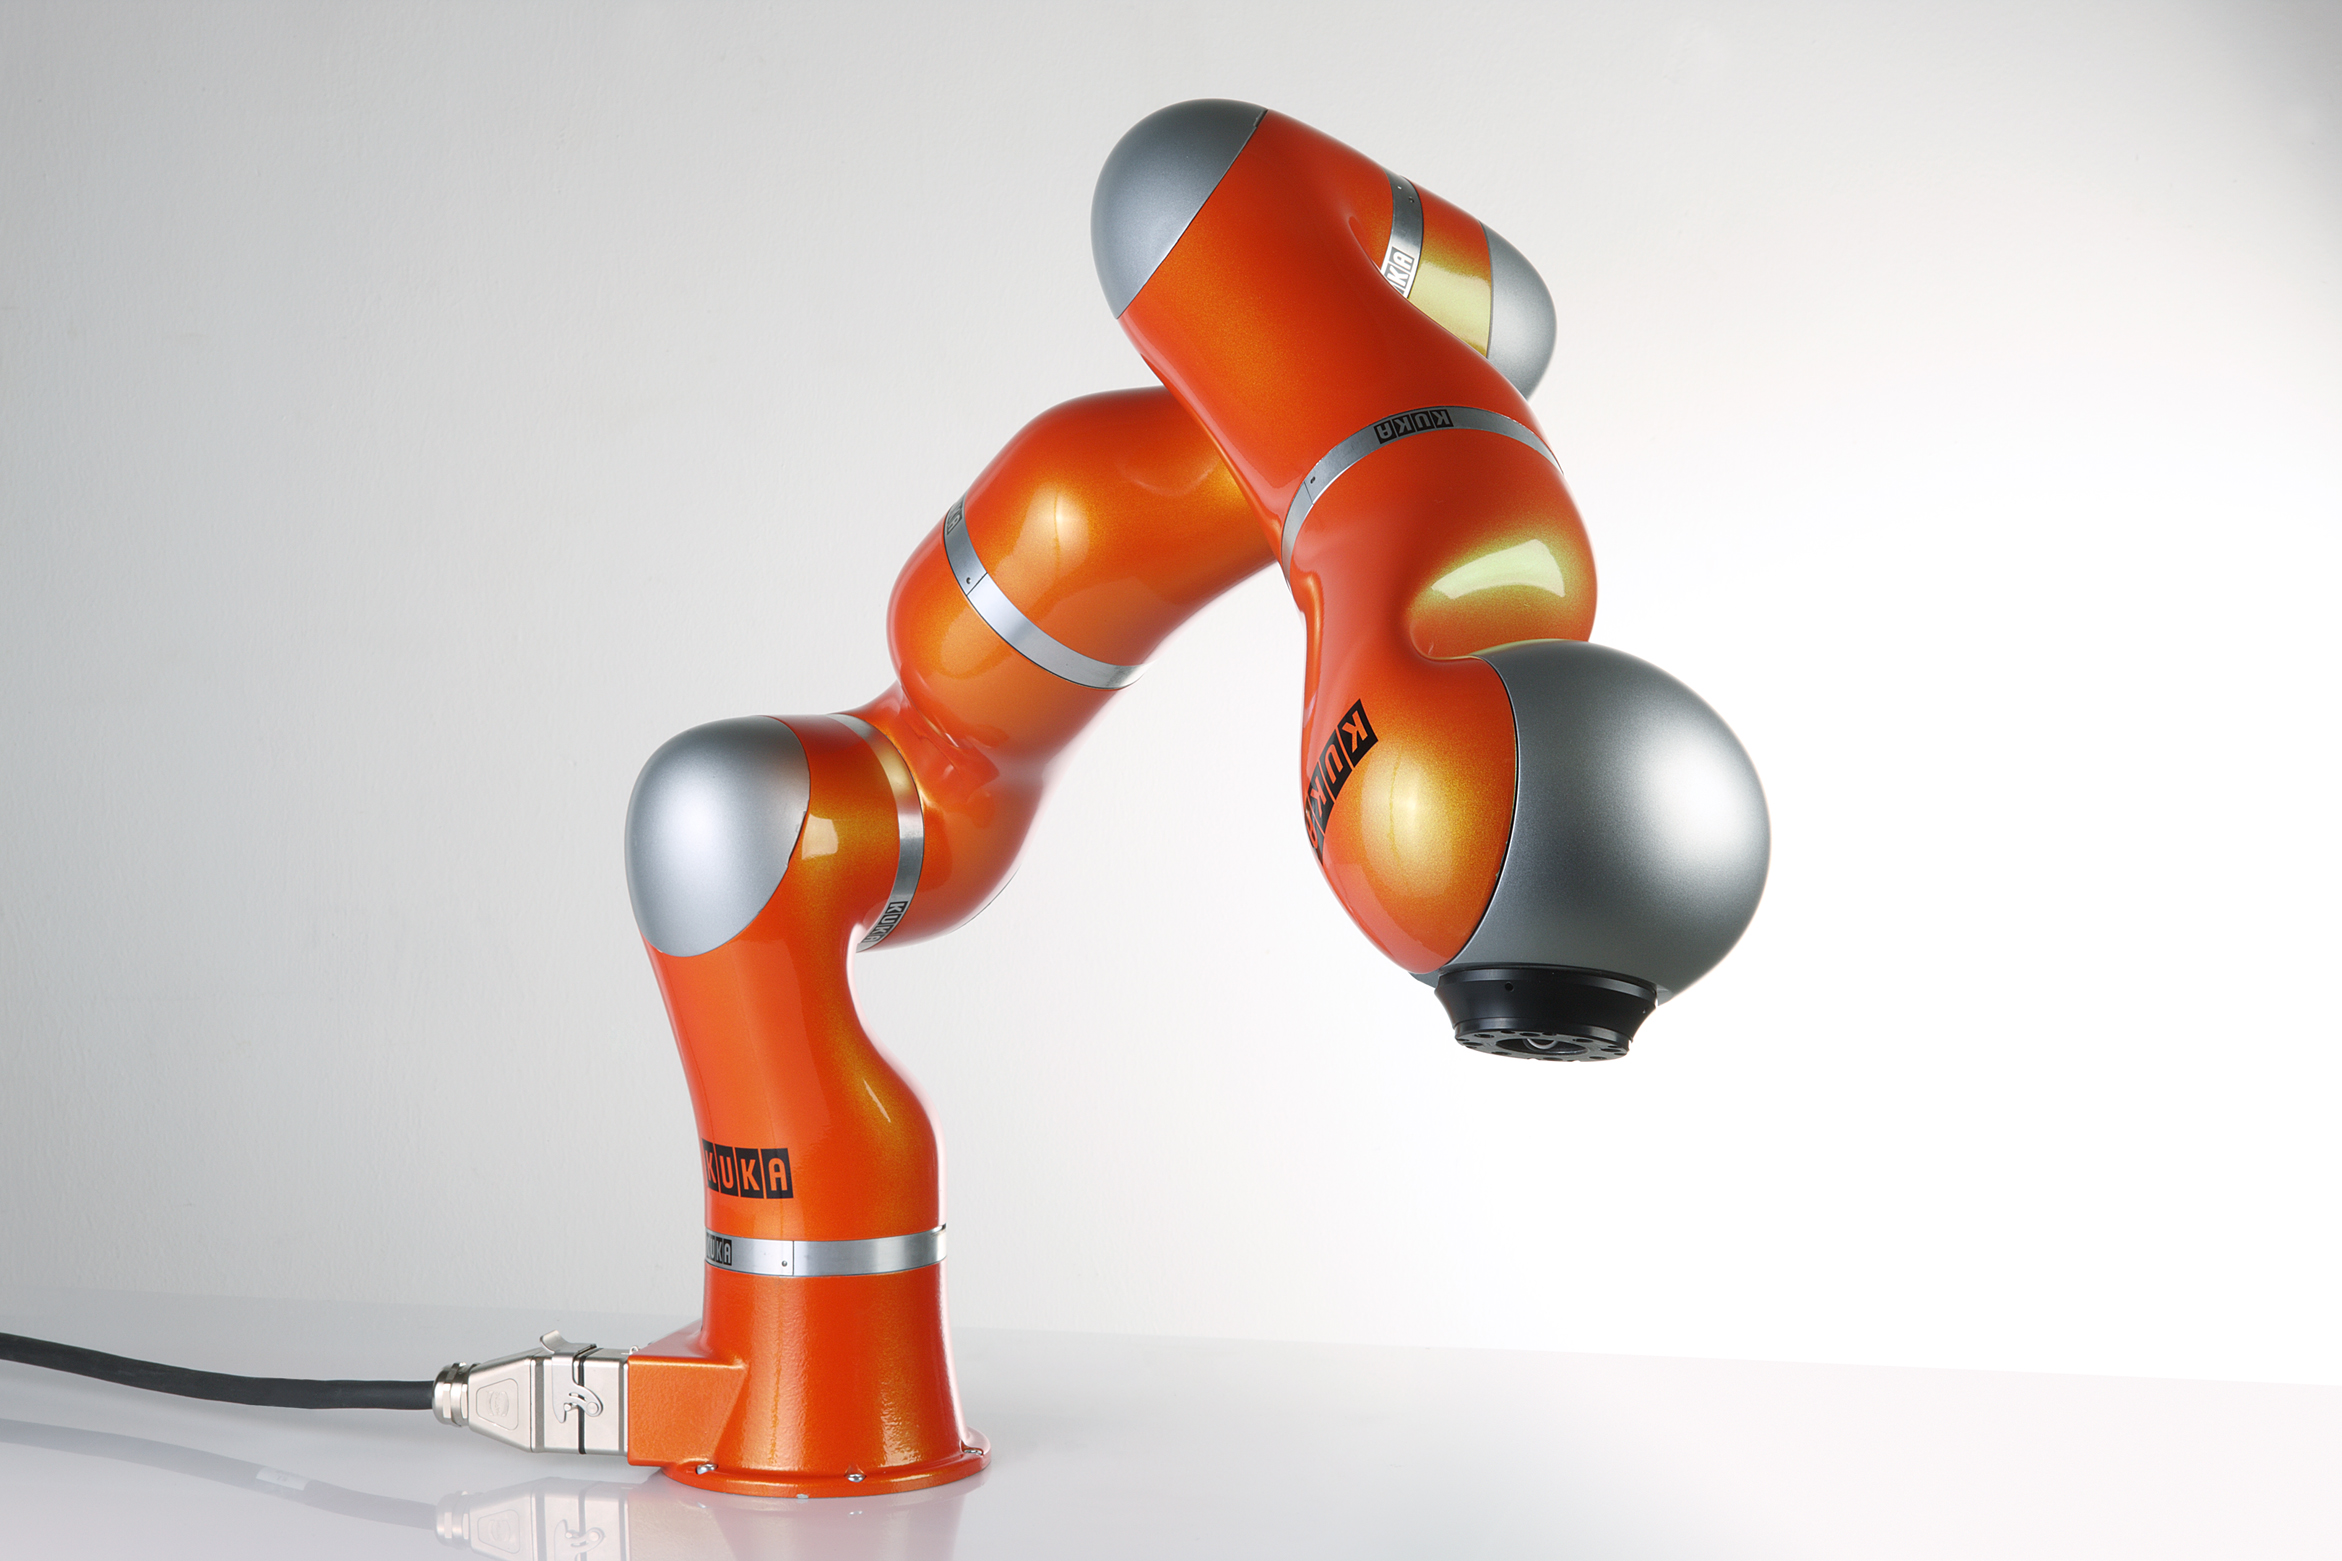
\includegraphics[scale=0.2]{KUKA.jpg}}
  node[anch, below = 15pt of kuka.east] (q_dq_feedback_anch){}
  node[anch, right = 20pt of q_dq_feedback_anch](q_dq_feedback_anch_2){}
  node[anch, below = 40pt of q_dq_feedback_anch_2](q_dq_feedback_anch_3){}
  node[anch, below = 29.555pt of op_space_inv_d](q_dq_feedback_anch_4){}
  node[anch, right = 20pt of hic.south](q_dq_feedback_anch_5){}

  node[anch, above = 20pt of kuka.east](force_feedback_anch_1){}
  node[anch, right = 35pt of force_feedback_anch_1](force_feedback_anch_2){}
  node[anch, below = 90pt of force_feedback_anch_2](force_feedback_anch_3){}
  ;
  
  \draw[->, thin] (high_level_p) -- node[pos=0.5]{$\vec{f}_{des}$}(hic);
  \draw[->, thin] (p_des_anchor_left) -- node[pos=0.5]{$\vec{p}_{des}$}(p_des_anchor_right);
  \draw[->, thin] (hic) -- node[pos=0.5]{$\vec{a}$}(op_space_inv_d);
  \draw[->, thin] (op_space_inv_d) -- node[pos=0.5]{$\vec{\tau}$}(kuka);
  \draw[-, thin] (q_dq_feedback_anch) -- node[pos=0.5]{$\vec{q}$,$\vec{\dot{q}}$} (q_dq_feedback_anch_2){};
  \draw[-,thin] (q_dq_feedback_anch_2) --(q_dq_feedback_anch_3){};
  \draw[->, thin] (q_dq_feedback_anch_3) -| (op_space_inv_d.south){};
  \draw[-, thin] (force_feedback_anch_1) -- node[pos=0.3]{$\vec{f}$}(force_feedback_anch_2) {};
  \draw[-, thin] (force_feedback_anch_2) -- (force_feedback_anch_3) {};
  \draw[->, thin] (force_feedback_anch_3) -| (hic.south) {};
  \draw[->, thin] (q_dq_feedback_anch_4) -| (q_dq_feedback_anch_5){};
  %% \draw[->, thin] (k_inverse) -- node[pos=0.4]{$\boldsymbol{\xi}_d$}(sum1);
  %% \draw[->, thin] (sum1) -- (projector);
  %% \draw[->, thin] (projector) -- (posctl);
  %% \draw[->, thin] (posctl.south) -- (sum2);
  %% \draw[->, thin] (wrench_ctl) -- (sum2);
  %% \draw[->, thin] (sum2) -- (robot.west);
  %% \draw[->, thin] (robot) |- node[pos=0.05, right = 0.05cm of robot]{$\vec{q}$} (transform);
  %% \draw[->, thin] (transform) -| node[near end]{$\boldsymbol{\xi}$} node[pos=0.9]{$-$}(sum1);
  %% \draw[->, thin](r) -- node [pos=0]{\Large $r$}(sum1);
  %% \draw[->, thin](sum1) -- node [pos=0.4]{\Large $e$}(controller);
  %% \draw[->, thin](controller) -- node [pos=0.3]{\Large $u$}(sum2);
  %% \draw[->, thin](w) -- node [pos=0]{\Large $w$}(sum2);
  %% \draw[->, thin](sum2) -- node[pos=0.3]{\Large $u_p$}(plant);
  %% \draw[->, thin](plant) -- node[pos = 0.7]{\Large $y$}(y);
  %% \draw[->, thin](n) -- node[pos=0]{\Large$n$}(sum3);
  %% \draw[->, thin](anchor1) -- (sum3);
  %% \draw[->, thin](sum3) -| node[pos=0.97] {$-$}(sum1);

\end{tikzpicture}
\end{document}
